\documentclass[../report.tex]{subfiles}

\begin{document}
\subsection{Các khái niệm trên tập mờ}
Xét tập $X$ không rỗng bất kì và $(X, d_X)$ là một
\textit{compact metrix space}. Một tập mờ $A$ trên tập $X$ được định nghĩa
như là một ánh xạ: $A: X \rightarrow [0, 1]$ và với mỗi điểm $x \in X$, giá trị 
$A(x)$ được gọi là \textit{membership degree} của $x$.

\textit{Support} của tập mờ $A$ được đĩnh nghĩa là lấy
\textit{topological closure} của $\{ x \in X | A(x) > 0 \}$.
Tập $\mathbb{F}(X)$ là tập các ánh xạ $A: X \rightarrow [0, 1]$ sao cho
$A$ là ánh xạ \textit{upper semi-continuous} và tập \textit{support} là
\textit{compact}. Tập $\mathbb{F}(X)$ có những điều kiện như vậy để có thể 
định nghĩa được một \textit{metric} trên đó.

Hơn nữa, với $\alpha \in (0, 1]$, một \textit{$\alpha$-cut} của A là tập
$[A]_{\alpha} = \{ x \in X | A(x) \ge \alpha\}$.
Một tập mờ $A$ được gọi là \textit{normal} nếu như $\exists x \in X, A(x) = 1$.
Nếu tập mờ $A$ là \textit{upper semi-continuous} thì mọi \textit{$\alpha$-cut} là 
một tập con \textit{đóng} của $X$.

Tập tất cả các tập tập mờ \textit{normal} và \textit{upper semi-continuous} trên 
tập $X$ được ký hiệu là $\mathbb{F}^1(X)$ và $\mathbb{F}_1^1(X)$ được định nghĩa là tập 
các \textit{số mờ} trên X -- là tập $\mathbb{F}_1^1(X) \subset \mathbb{F}^1(X)$
các tập mờ mà trong đó mọi \textit{$\alpha$-cut} đều là tập con
\textit{topologically connected} của $X$.

\subsection{Metric trên $\mathbb{F}(X)$}
Metric trên $\mathbb{F}(X)$ thường được định nghĩa dựa vào \textit{Hausdorff metric}
$D_X$ giữa hai tập con $E, F \in \mathbb{K}(X)$ TODO, trong đó $\mathbb{K}(X)$ là 
tập các tập con đóng của X. Đây là lý do tại sao ta chỉ xét các tập mờ
\textit{upper semi-continuous}, bởi vì khi đó mọi \textit{$\alpha$-cut} đều là các
tập đóng. \textit{Hausdorff metric} được định nghĩa như sau: 
$$
D_X(E, F) = \inf \{\varepsilon > 0 | E \subset U_{\varepsilon}(F), F \subset U_{\varepsilon}(E) \}
$$
trong đó
$$
U_{\varepsilon}(E) = \{ x \in X | D(x, E) < \varepsilon \}
$$
và
$$
D(x, E) = \inf_{e \in E} d_X(x, e)
$$
Từ đó ta có thể định nghĩa metric $d_{\infty}$
(còn được gọi là \textit{supremum metric}) như sau: 
$$
d_{\infty} = \sup_{\alpha \in (0, 1]} D_X([E]_{\alpha}, [F]_{\alpha})
$$
với mọi $E, F \in \mathbb{F}^1(X)$

\subsection{Hệ động học}
Một hệ động học (rời rạc) là một bộ $(X, f)$ trong đó $X$ là một \textit{metric space}
và $f: X \rightarrow Y$ là một ánh xạ liên tục. 

Tại một điểm cố định bất kỳ $x \in X$, ta xét một dãy $\{ f^n(x) \}_{n \in \mathbb{N}}$
bao gồm các giá trị được định nghĩa quy nạp bởi $f^0(x) = x$, $f^1(x) = f(x)$
và $f^{n + 1} (x)$ = $f(f^n(x))$ với mọi $n \in \mathbb{N}$. Dãy giá trị này còn được gọi
là \textit{quỹ đạo} của $x$ qua ánh xạ $f$. Điểm từ tập $X$ có thể được mô tả bằng các 
tính chất của quỹ đạo. Ví dụ, điểm $x \in X$ được gọi là điểm cố định (\textit{fixed point})
của $f$ nếu như $f(x) = x$. Điểm $x \in X$ được gọi là điểm tuần hoàn của $f$ nếu như tồn tại 
$n \in \mathbb{N}, n > 0$ sao cho $f^n(x) = x$. Ví dụ dưới đây mô tả một hệ mà thay đổi 
nhỏ giá trị khởi tạo có thể dẫn đến thay đổi lớn hành vi của hệ động học. 

Ví dụ, xét một \textit{tent map} $T$, trong đó $T: [0, 1] \rightarrow [0, 1]$ được định 
nghĩa bởi $T(x) = 2x$ với $x \in [0, 1/2)$ và $T(x) = 2(1 - x)$ với 
$x$ thuộc giá trị còn lại. 

\begin{figure}[H]
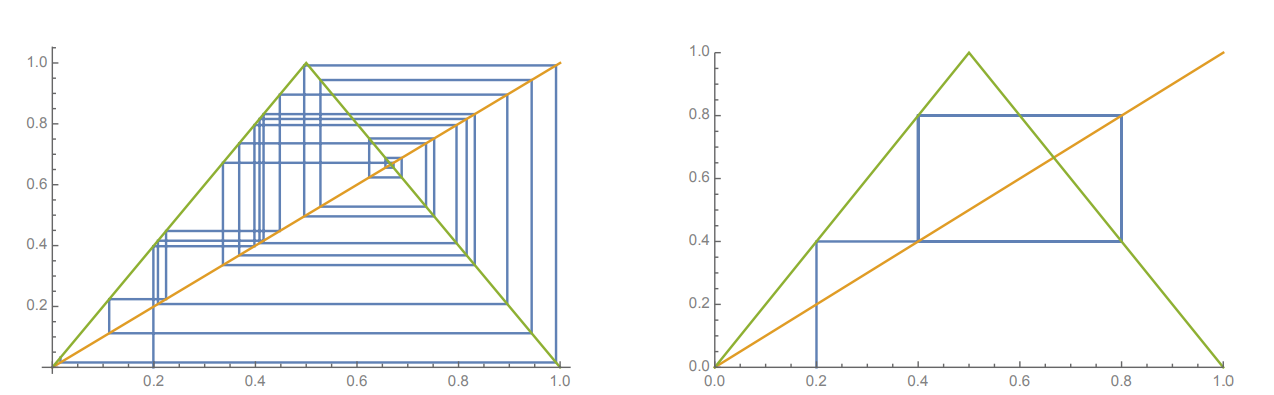
\includegraphics[width=\textwidth]{figures/tent-map.png}
\caption{50 vòng lặp, $x_0 = 0.199$ (hình bên trái), $x_0 = 0.2$ (hình bên phải)}
\label{fig:1}
\end{figure}

Trong hình \ref{fig:1}, nếu ta lấy $x_0 = 0.199$ là giá trị khởi tạo, quỹ đạo 
sinh ra là phức tạp. Còn với $x_0 = 0.2$ quỹ đạo trở nên tuần hoàn. 

\subsection{Hệ động học mờ}
Xét $(X, f)$ là một hệ động học rời rạc. Biểu thức:
$$
(z_f(A))(x) = \sup_{y \in f^{-1} (x)} \{ A(y) \}
$$
định nghĩa duy nhất một ánh xạ $z_f: \mathbb{F}^1(X) \rightarrow \mathbb{F}^1(X)$. 
Ánh xạ $z_f$ là một ánh xạ mờ hóa (hay mở rộng Zadeh)
của ánh xạ $f: X \rightarrow X$. 
Hơn nữa, $z_f$ là liên tục trong $(\mathbb{F}^1(X), \tau_{\infty})$
khi và chỉ khi $f$ là liên tục, trong đó $\tau_{\infty}$ là \textit{topology}
sinh bởi metric $d_{\infty}$. 

Đồng thời, nguyên lý mở rộng của Zadeh có liên hệ mật thiết với 
một mở rộng tự nhiên khác $(\mathbb{K}(X), s_f)$ của $(X, f)$, trong đó
$s_f: \mathbb{K}(X) \rightarrow \mathbb{K}(X)$ được định nghĩa bởi 
$s_f(C) = f(C)$ với mọi $C \in \mathbb{K}(X)$.

Thật vậy, $[z_f(A)]_{\alpha} = s_f([A]_{\alpha}) = f([A]_{\alpha})$ 
với mọi $A \in \mathbb{F}^1(X)$ và $\alpha \in (0, 1]$.

\subsection{Piecewise Linear Function}
Dưới đây chúng ta sẽ mô tả thuật toán cho các hàm \textit{piecewise linear}
$f: [0, 1] \rightarrow [0, 1]$ được cho bởi hữu hạn các điểm
$(c_i, s_i) \in [0, 1] \times [0, 1]$ với $i = 1,\cdots, l$, là một 
hàm mà $c_1 = 0, c_l = 1$ và $f(c_i) = s_i$ với $i = 1, \cdots, l$ và 
$f|_{[c_i, c_{i + 1}]}$ là các ánh xạ tuyến tính với $i = 1, \cdots, l - 1$.
Các điểm $c_i$ được gọi là các điểm \textit{turning point}. Với $f$ được định nghĩa như vậy thì hiển nhiên $f$ là liên tục. Tuy nhiên thuật toán áp 
dụng được mô tả dưới đây có thể sử dụng cho các hàm không liên tục. Điểm 
khác biệt duy nhất với các hàm đó là được mô tả bằng tập các cặp của các 
cặp giá trị $(c_i, s_i)$, với mỗi cặp của các cặp giá trị mô tả một 
đoạn thẳng. 

Bởi vì tập các hàm \textit{piecewise linear} là \textit{dense} trong tập 
các ánh xạ liên tục nên ta có thể xấp xỉ một ánh xạ liên tục bất kì với 
sai số nhỏ tùy ý. Hơn nữa tính toán trên các ánh xạ 
\textit{piecewise linear} là đơn giản hơn và có thể tính chính xác. Vì thế ở đây ta chỉ xét 
thuật toán áp dụng trên các ánh xạ này. 

\end{document}
